\chapter{Material und Methoden}

In diesem Kapitel werden die Materialien und Methoden vorgestellt mit denen die Messungen durchgeführt werden.


\section{Testplattform}
\subsection{HPC Cluster Server}
\subsection{Multicore Computer}
TEST

\section{Metriken als Symptome}

Als Metriken werden in dieser Bachelorarbeit definierte Aktivitäten wie beispielsweise Cache Zugriffe interpretiert. Diese Aktivitäten werden mithilfe von Hardware Perfomance Countern dokumentiert und als Symptome behandelt. Das Perfomance Application Programming Interface (kurz: PAPI) dient dem leichteren Auslesen dieser Perfomance Counter.



\subsection{Hardware Perfomance Counter}

Hardware Perfomance Counter sind spezielle Mehrzweckregister die in modernen Prozessoren
eingebaut sind. Diese Register werden von der on-chip Performance Monitoring Unit (kurz:
PMU) verwaltet und beschrieben.
\cite{PMU}
Das Ziel der PMU ist das Zählen und somit Dokumentieren von Events, wie z.B. Zyklen, Cache Misses oder Floating Point Operations, die im folgenden als Symptome definieren.

Diese Events können in Hardware Events (CPU-Cycles, Instructions, Cache Zugriffe etc,) und Software Events (Page Faults, Context Switche,..) unterschieden werden.

Im Allgemeinen besteht die Hardware zum Zählen der Events aus zwei Komponenten: 

Zum einen die Perfomance Event Select Registers

Diese geben an welche Events überwacht und wie gemessen wird.
Und Event Counters, die als Zielregister für die Werte fungieren.

\begin{figure}[ht]
	\centering
	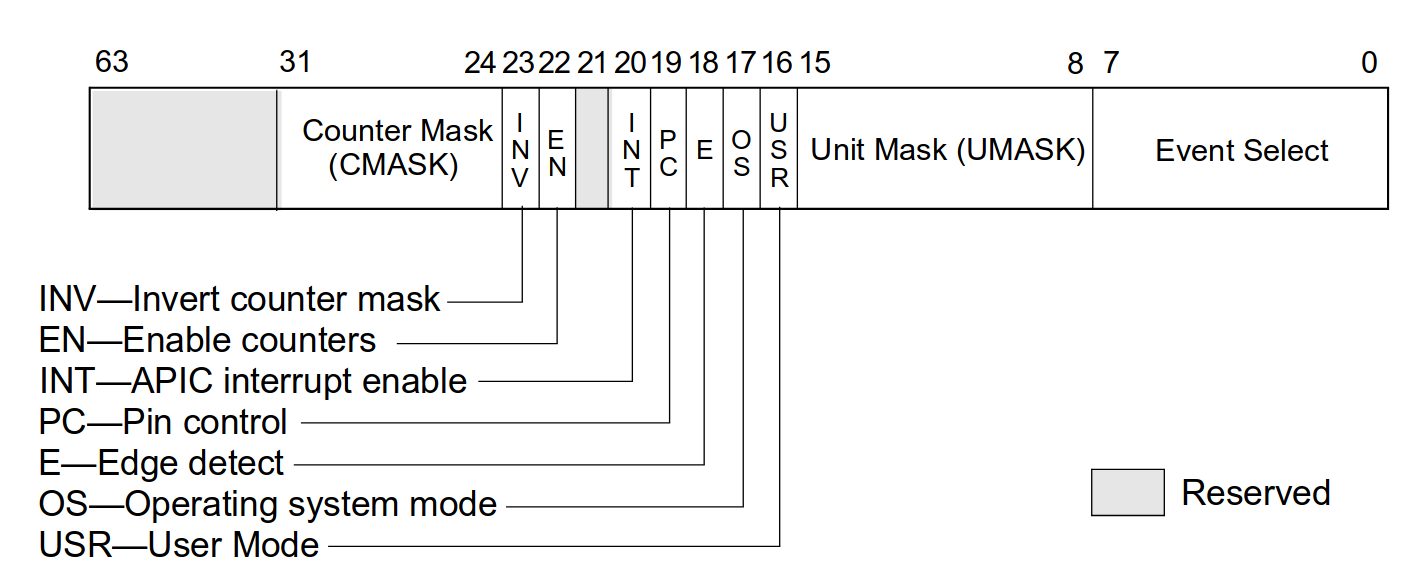
\includegraphics[width=0.8\textwidth]{MSR.png}
	\caption{Intel IA32PERFEVTSELxMSRs (https://software.intel.com/sites/default/files/managed/39/c5/325462-sdm-vol-1-2abcd-3abcd.pdf)}
	\label{fig1}
\end{figure}

Man unterscheidet gemäß Intel zwischen drei Typen von Perfomance Countern:
\begin{itemize} 
	
\item Fixed function counters 
\item General purpose perfomance counters
\item Precise-event based sampling

\end{itemize}

Entwicklung der Perfomance Counter

\begin{figure}[ht]
	\centering
	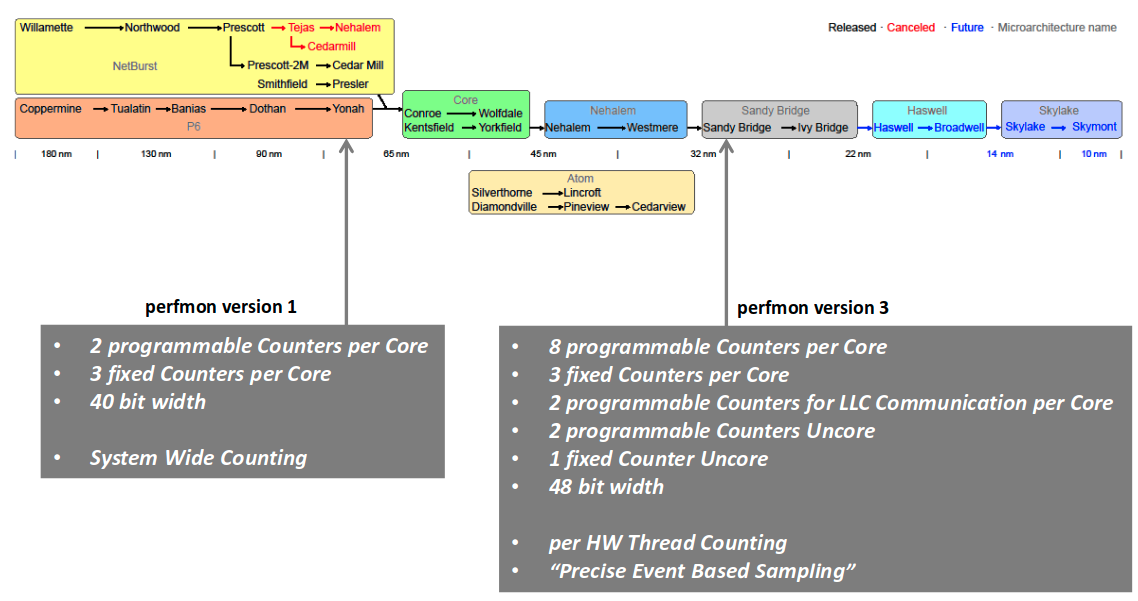
\includegraphics[width=0.8\textwidth]{EvoHPC.png}
	\caption{https://www.inf.ethz.ch/personal/markusp/teaching/263-2300-ETH-spring13/slides/11-perfcounters.pdf}
	\label{fig2}
\end{figure}

Ein Pentium III Prozessor (1999) besitzt zwei Hardware Perfomance Counter, wohingegen ein
aktueller Prozessor wie der Intel Xeon E5-2620 (2014) 634 Perfomance Counter zur Verfügung
stellt, wie der Tabelle im Anhang entnommen werden kann.
\cite{Xeon}

Perfomance Counter werden üblicherweise benutzt um in Abhängigkeit einer Anwendung Hardware auf Engpässe, sogenannte Bottle Necks zu untersuchen. Bottle Necks können typischerweise zu geringer Speicher, geringer Netzwerkdurchsatz oder eine überlastete CPU sein. \cite{HPC} 

Ein Beispiel für die klassische Verwendung ist folgender Programmcode.

\begin{figure}[ht]
	\centering
	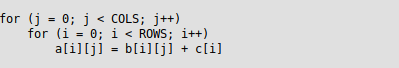
\includegraphics[width=0.8\textwidth]{graphic/Code.png}
	\caption{http://perfsuite.ncsa.illinois.edu/publications/LJ135/x35.html}
	\label{fig3}
\end{figure}

Bei einem unoptimierten Compiler, würden die benachbarten Datenelemente nie nacheinander zugegriffen werden. Messungen an der NCSA Illinois zeigen, dass dies zu einer höheren Anzahl von L2-Cache Misses (212 665 026) führt.


Wenn man allerdings die verschachtelten Schleifen umändert, dass die Matrizen row-by-row basiert durchgegangen werden würde. was der Intel ICC Compiler macht, dann sinken um 11,89 Prozent die L2-Cache Misses auf 25 287 572. Gleichzeitig erfolgt die Berechnung 10-Mal so schnell.
\cite{CacheUnfriendly}


\subsection{Perfomance Application Programming Interface}

Die University of Tennessee entwickelt das Performance Application Programming Interface
(kurz: PAPI) um einen leichteren Zugriff auf perfomance counter anzubieten. Das einheitliche
PAPI-Interface bietet Entwicklern eine Abstraktion der nativen Interfaces und somit eine
vereinfachte Entwicklung. 
PAPI unterstützt alle aktuellen Intel und AMD x86 sowie x8664 Prozessoren (CPU). Durch die
Erweiterung PAPI CUDA wird der Zugriff auf perfomance counter von nVidia Grafikkarten (GPU)
erweitert.
Es wird zwischen high-level interface sowie low-level interface unterschieden. Das high-level
interface bietet einen einfachen sowie schnellen Zugriff, wohingegen das low-level interface
mehr Kontrolle und einen detailliertes Vorgehen erlaubt. In dieser Arbeit wird vor allem das low
level interface benutzt. Informationen über die Implementierungsarbeit ist in Abschnitt 4 zu
finden.
Jede Plattform (CPU, GPU,..) besitzt sogenannte native events, die aus den unterstützen
hardware Performance Countern abgeleitet werden. Die Namen dieser events sind
plattformabhängig. Durch generische preset events abstrahiert PAPI diese nativen events und
ermöglicht dem Entwickler eine einheitliche Sicht ohne exakte Kenntnisse der native events zu
fordern. Sofern ein preset event nicht verfügbar ist versucht PAPI dieses von anderen events
abzuleiten, z.B. Total Number of L2 Cache Misses = L2 Cache Access - L2 Cache Hits.
Die Konfiguration der Events wird durch EventSets ermöglicht. Diese bestehen aus einem oder
mehreren Events und klassifizieren wie die events gemessen werden sollen, z.B. ob der code
im user space oder kernel space ablaufen soll.

\section{Physikalische Fehlerinjektion}

TEST

\subsection{Simulation von defekten CPU-Cores}
TEST

\subsection{Simulation von unzureichender Spannungsversorgung}
TEST
\subsection{Manipulation der Taktfrequenz}
TEST

\subsection{Manipulation der Speicherfrequenz}
TEST

\section{Softwarebasiere Fehlerinjektion}

\subsection{Fehlerinjektion in POSIX Bibliothek}
TEST
\subsection{Fehlerinjektion im Linux Kernel}
TEST

\subsection{Fehlerinjektion zur Laufzeit}
TEST

\section{Benchmarks}
TEST


\subsection{Rodinia Benchmark Suite}
TEST


\subsection{Eigene Benchmarks}
TEST
